\section{Preliminaries}
\subsection{Citing MetaOmics}
MetaOmics software suite implements many meta-analysis methods from different authors. 
Please cite appropriate papers if you use MetaOmics,
by which the authors will receive professional credits for their work.

\begin{itemize}

\item MetaOmics software suite itself can be cited as: 

\begin{itemize}
\item Ma, T., Huo, Z., Kuo, A., Zhu, L., Fang, Z., Zeng, X., Lin, C.-W., Liu, S., Wang, L., Rahman, T., Chang, L.-C., Kim, S., Li, J., Park, Y., Song, C., Oesterreich, S., Sibille, E. and Tseng, G. C. MetaOmics: Comprehensive Analysis Pipeline and Browser-based Software Suite for Transcriptomic Meta-Analysis.
\end{itemize}

\item Review, comparative papers and published R packages:
\begin{itemize}
\item \bibentry{tseng2012comprehensive}.
\item \bibentry{chang2013meta}.
\item \bibentry{wang2012r}.
\end{itemize}

\item MetaQC: 
\begin{itemize}
\item (MetaQC) \bibentry{kang2012metaqc}.
\end{itemize}

\item MetaDE: 
\begin{itemize}
\item (Fisher) \bibentry{fisher1925statistical}.
\item (AW-Fisher) \bibentry{li2011adaptively}.
\item (AW-Fisher) \bibentry{huo2017p}.
\item (REM/FEM) \bibentry{choi2003combining}.
\item (rOP) \bibentry{song2014hypothesis}.
\item (minMCC) \bibentry{lu2009biomarker}.
\item (Stouffer) \bibentry{stouffer1949american}
\item (RankProd) \bibentry{hong2006rankprod} 
\end{itemize}

\item MetaPath: 
\begin{itemize}
\item (MAPE) \bibentry{shen2010meta}.
\item (CPI) \bibentry{fang2016cpi}.
\end{itemize}

\item MetaNetwork: 
\begin{itemize}
\item (MetaDCN) \bibentry{zhu2016metadcn}.
\end{itemize}

\item MetaPredict: 
\begin{itemize}
\item (MetaKTSP) \bibentry{Kim2016}.
\end{itemize}

\item MetaClust: 
\begin{itemize}
\item (MetaSparseKmeans) \bibentry{huo2016meta}.
\end{itemize}

\item MetaPCA: 

\begin{itemize}
\item (MetaPCA) \bibentry{kim2017meta}.
\end{itemize}

\end{itemize}



\subsection{How to start MetaOmics}

The full instruction of how to install and start MetaOmics software suite is also available at \url{https://github.com/metaOmics/metaOmics}.
There are two ways to start the metaOmics software:
via R software, or via docker.


\subsubsection{Start from R}

\textbf{Requirement:}
\begin{itemize}
\item R $>=$ 3.3.1
\item Shiny $>=$ 0.13.2
\end{itemize}

\noindent\textbf{Note:}

\begin{itemize}
\item We recommend users to use R 3.3 to implement our tool. If you are using R 3.4 (released on 4/24/2017), you may encounter errors in installing dependencies of the modules. You can manually install the dependencies by running the following commands in R:

\textit{install.packages(c(\textquotesingle GSA\textquotesingle, \textquotesingle combinat\textquotesingle, \textquotesingle   samr\textquotesingle   , \textquotesingle   survival\textquotesingle   , \textquotesingle   cluster\textquotesingle   , \textquotesingle   gplots\textquotesingle   , 
  \textquotesingle   ggplot2\textquotesingle   , \textquotesingle   irr\textquotesingle   , \textquotesingle   shape\textquotesingle   , \textquotesingle   snow\textquotesingle   , \textquotesingle   snowfall\textquotesingle   , \textquotesingle   igraph\textquotesingle   , \textquotesingle   doMC\textquotesingle   , \textquotesingle   PMA\textquotesingle   ))
  }

\textit{source(\textquotesingle   https://bioconductor.org/biocLite.R\textquotesingle   )  }

\textit{biocLite(c(\textquotesingle   multtest\textquotesingle   , \textquotesingle   Biobase\textquotesingle   , \textquotesingle   edgeR\textquotesingle   , \textquotesingle   DESeq2\textquotesingle   , \textquotesingle   impute\textquotesingle   , 
  \textquotesingle   limma\textquotesingle   , \textquotesingle   AnnotationDbi\textquotesingle   , \textquotesingle   ConsensusClusterPlus\textquotesingle   , \textquotesingle   genefilter\textquotesingle   , \textquotesingle   GSEABase\textquotesingle   , \textquotesingle   Rgraphviz\textquotesingle   ))
  }

\item For Windows, users need to run the following command in R to install the package \textquotesingle doMC\textquotesingle:

\textit{install.packages(\textquotesingle doMC\textquotesingle, repos=\textquotesingle http://R-Forge.R-project.org\textquotesingle)}

\end{itemize}

 

\noindent\textbf{How to install the software:}
\begin{itemize}
\item At MetaOmics home page \url{https://github.com/metaOmics/metaOmics}, clone the project by
clicking on ``Clone or download" and extract to a working directory, 
or type in the following in command line:

\textit{git clone} \url{https://github.com/metaOmic/metaOmics}
\end{itemize}

\noindent\textbf{How to start the software:}

\begin{enumerate}
\item Open R 
\item Set the working directory such that metaOmics folder included. 

\textit{install.packages(\textquotesingle shiny\textquotesingle)}

\textit{shiny::runApp(\textquotesingle metaOmics\textquotesingle, port=9987, launch.browser=T)}
\end{enumerate}


\subsubsection{Run from docker image:}

\begin{enumerate}
\item Install docker (\url{https://www.docker.com}).
\item In terminal

\textit{docker pull metaomics/app}

\textit{docker run --rm --name metaOmics -p 3838:3838 metaomics/app}

\end{enumerate}


\subsection{MetaOmics setting page}
\label{sec:setting}
After starting MetaOmics, 
the first page is the MetaOmics setting page as shown in Figure~\ref{fig:GUIsetting}.  
There are four tabs on the top of this page (See Figure~\ref{fig:GUIsetting} {\color{red} (1)}), 
which will direct users to specific functional modules of the software including ``Setting", ``Preprocessing", ``Saved Data" and ``Toolsets".
Below these tabs is a {\bf Welcome to MetaOmics} section, which briefly introduces the software and other information about the authors and maintainers.
Further below, there are two sections: {\bf Session Information} and {\bf Directory for Saving Output Files} (See Figure~\ref{fig:GUIsetting} {\color{red} (2)}).
By clicking ``$\ldots$",
users can set working directory, in which all the meta-analysis results will be saved.
The current working directory is displayed on the top right corner (See Figure~\ref{fig:GUIsetting} {\color{red} (3)}).
There is one more section with the header {\bf Toolsets} (See Figure~\ref{fig:GUIsetting} {\color{red} (4)}),
where users can click the blue button to install the desired modules if the ``Status" shows ``not installed".
If the packages are already installed, an icon of ``checked installed" will show up in ``Status".
%Otherwise, users can install individual package by clicking install blue button.
The installation progress may take up to a few minutes for each module.
A notification icon will pop up at the bottom right corner upon finishing the installation process. 
After the modules are installed, users need to restart the MetaOmics software suite so that the Shiny application interface is updated with the installed modules.
(See Figure~\ref{fig:GUIsetting} {\color{red} (5)}) shows the current active dataset, 
which is introduced in Section~\ref{sec:procedure}~\ref{sec:active}. 
 
\begin{figure}[H]
\begin{center}
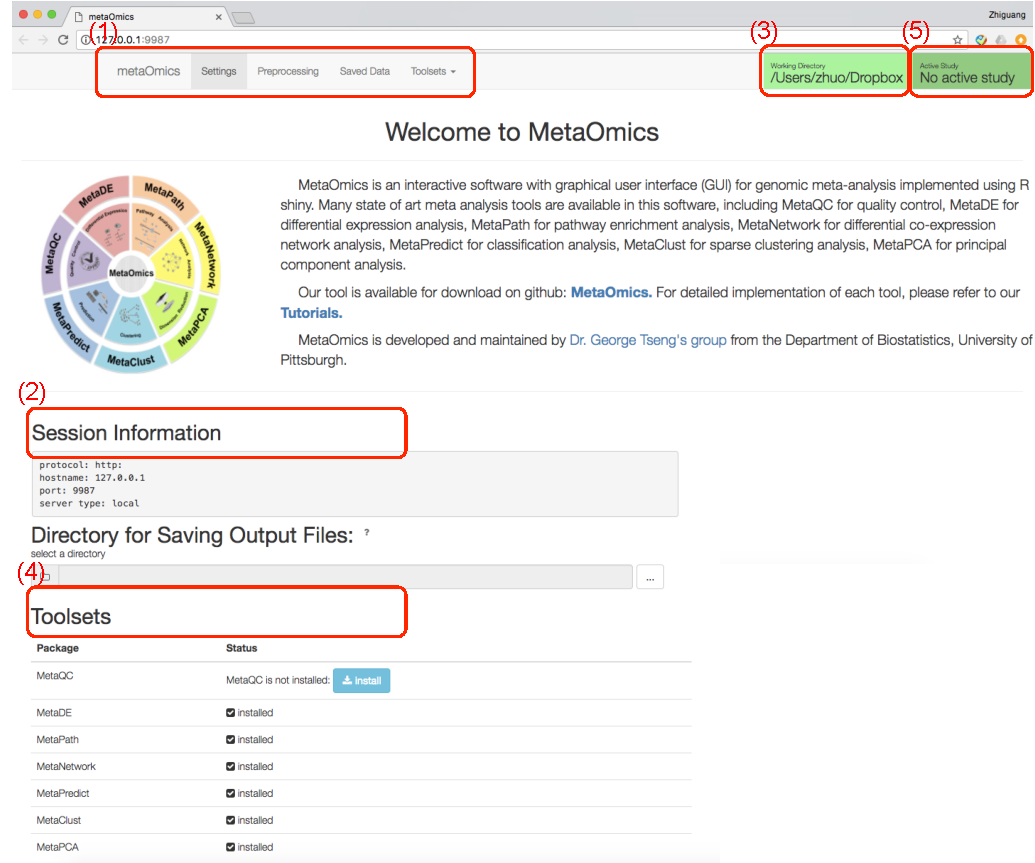
\includegraphics[scale=0.9]{./figure/preprocessing/GUIsetting}
\caption{MetaOmics software suite GUI setting page}
\label{fig:GUIsetting}
\end{center}
\end{figure}


\subsection{Question and bug report}

If you encounter errors or bugs, please report to the maintainer Tianzhou Ma $<$\url{tim28@pitt.edu}$>$.


 
